\section{An GPU Programming Example: Stencil Computation}\ref{sec:stencil_example}


\subsection{Problem: Heat flow in two-dimensional area}


\par
Heat flows in objects according to local temperature differences, as if seeking local equilibrium.
The following example defines a rectangular area with two always-warm sides (temperature 70 and 85), two cold sides (temperature 20 and 5) and a cold disk at the center.
Because of heat diffusion, temperature of neighboring patches of the area is bound to equalize, changing the overall distribution over time, as shown in Fig.~\ref{fig:heat_montage}.

\begin{figure}[!htbp]
\centering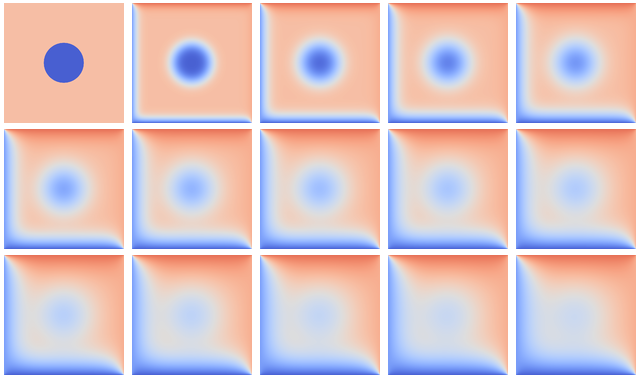
\includegraphics[width=0.7\textwidth]{fig_problem/heat_montage.png}
\caption{Over time, the temperature distribution in the rectangular area progresses from the initial state toward an end state where upper triangle is warm and lower is cold. The average temperature tends to (70+85+20+5)/4=45.}\label{fig:heat_montage}
\end{figure}


% ---------------------------------------------------------------------- %


\subsection{Technique: Stencil computation}


\par
Heat transfer in the system mentioned above is governed by the partial differential equation (PDE) describing local variation of the temperature field in time and space.
That is, the rate of change of the temperature field $u(x,y,t)$ over two spatial dimensions $x$ and $y$ and time $t$ (with rate coefficient $\alpha$) can be modelled via the equation
\begin{equation}
    \frac{\partial u}{\partial t} = \alpha \Big(\frac{\partial^2u}{\partial x^2} + \frac{\partial^2u}{\partial y^2}\Big) \,. \label{eq:heat_diffusion_pde}
\end{equation}

 
\par
The standard way to numerically solve the differential equations is to discretize them, $i.e.$, to consider only a set/grid of specific area points at specific moments in time.
That way, partial derivatives $\partial u$ are converted into differences between adjacent grid points $u^m(i,j)$, with $m$, $i$, $j$ denoting time and spatial grid points, respectively.
Temperature change in time at a certain point can now be computed from the values of neighboring points at earlier time; the same expression, called~\textbf{stencil} (shown in Fig.~\ref{fig:stencil}), is applied to every point on the grid.


\begin{figure}[!htbp]
\centering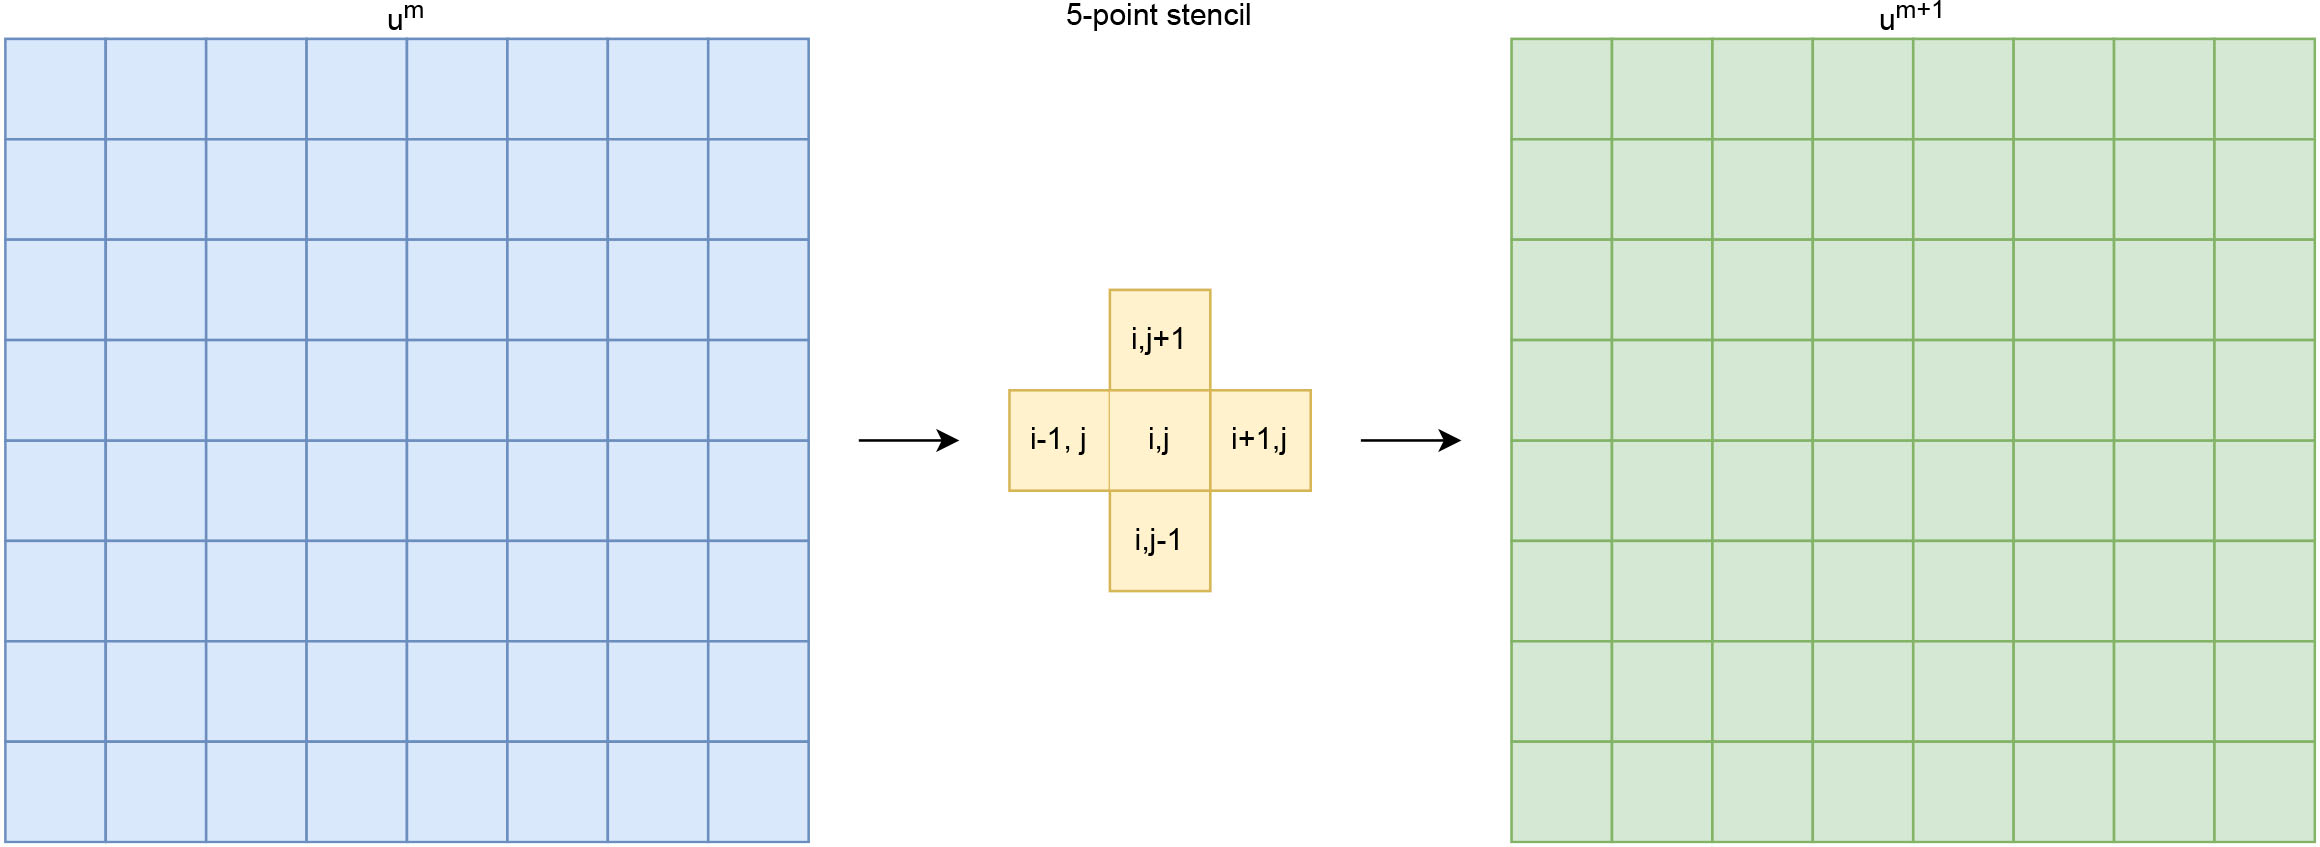
\includegraphics[width=0.8\textwidth]{fig_problem/stencil.jpg}
\caption{This simplified model uses an 8x8 grid of data in light blue in state $m$, each location of which has to be updated based on the indicated 5-point stencil in yellow to move to the next time point $m+1$.}\label{fig:stencil}
\end{figure}


\par
It should be mentioned that stencil computation is a common occurrence in solving numerical problems.
One obvious choice for stencil computations is the convolution operation.
Using the stencil convolution operation to solve the PDE for the heat diffusion, we will have several technical considerations.


\subsubsection{How fast and/or accurate can the solution be?}


\par
Spatial resolution of the temperature field is controlled by the number/density of the grid points.
As the full grid update is required to proceed from one time point to the next, stencil computation is the main target of parallelization (on CPU or GPU).
Moreover, in many cases the chosen time step cannot be arbitrarily large, otherwise the numerical differentiation will fail, and dense/accurate grids imply small time steps (see the equations below), which makes efficient spatial update even more important.


\par
One option for stencil expression and time-step limit is described below.
The differential equation shown in Eq.~\ref{eq:heat_diffusion_pde} can be discretized using different schemes.
For this example, the temperature values at each grid point $u^m(i,j)$ are updated from one time point ($m$) to the next ($m+1$), using the following expressions:
\begin{equation}
    u^{m+1}(i,j) = u^m(i,j) + \Delta t \alpha \nabla^2 u^m(i,j) \,,
\end{equation}
where 
\begin{equation}
    \nabla^2u = \frac{u(i-1,j)-2u(i,j)+u(i+1,j)}{(\Delta x)^2} + \frac{u(i,j-1)-2u(i,j)+u(i,j+1)}{(\Delta y)^2}\,,
\end{equation}
and $\Delta x$, $\Delta y$, $\Delta t$ are step sizes in space and time, respectively.
Time-update schemes also have a limit on the maximum allowed time step $\Delta t$.
For the current scheme, it is equal to
\begin{equation}
    \Delta t_{max} = \frac{(\Delta x)^2(\Delta y)^2}{2\alpha((\Delta x)^2+(\Delta y)^2)}\,.
\end{equation}


\subsubsection{What to do with area boundaries?}


\par
Naturally, stencil expression can’t be applied directly to the outermost grid points that have no outer neighbors. This can be solved by either changing the expression for those points or by adding an additional layer of grid that is used in computing update, but not updated itself – points of fixed temperature for the sides are being used in this example.


\subsubsection{How could the algorithm be optimized further?}


\par
In an earlier subsection~\ref{sec:memory_optimization}, importance of efficient memory access was already stressed.
In the following examples, each grid point (and its neighbors) is treated mostly independently; however, this also means that for 5-point stencil each value of the grid point may be read up to 5 times from memory (even if it’s the fast GPU memory).
By rearranging the order of mathematical operations, it may be possible to reuse these values in a more efficient way.


\par
Another point to note is that even if the solution is propagated in small time steps, not every step might actually be needed for output.
Once some local region of the field is updated, mathematically nothing prevents it from being updated for the second time step – even if the rest of the field is still being recalculated – as long as $t=m-1$ values for the region boundary are there when needed.
Of course, this is more complicated to implement and would only give benefits in certain cases.


% ---------------------------------------------------------------------- %


\subsection{Sequential and thread-parallel program in C++}


\par
Source files of the code examples presented for the rest of this section are available in the~\textbf{\textcolor{brown}{content/examples/stencil/}} subdirectory of this repository~\cite{gpu-programming-examples}.
You can use Git to download them to your home directory on the cluster.
It should be noted that do not forget to git pull for the latest updates if you already have the content from the first day of this workshop.
\lstinputlisting[language=bash, firstline=1, lastline=2, label={lst:13_heat_diffusion_stencil_path}, xleftmargin=0.05\textwidth, xrightmargin=0.05\textwidth]{code_examples/13_heat_diffusion_stencil_path.pbs}


\par
The general structure (main function), the default parameter values for the problem model, and the stencil update scheme of this program is shown in List~\ref{lst:13_heat_diffusion_stencil_cpu_main}, List~\ref{lst:13_heat_diffusion_stencil_cpu_params}, and List~\ref{lst:13_heat_diffusion_stencil_cpu_update}, respectively. 
If we assume the grid point values to be truly independent for a single time step, stencil application procedure may be straighforwardly written as a loop over the grid points, as shown in List~\ref{lst:13_heat_diffusion_stencil_cpu_update}.
The CPU-thread parallelism can then be enabled by a single OpenMP~\textbf{\textcolor{red}{\#pragma}} shown in the 26$^{th}$ line in List~\ref{lst:13_heat_diffusion_stencil_cpu_update}.


\lstinputlisting[language=c++, caption={The general structure (main function) for the head diffusion program in C++.}, label={lst:13_heat_diffusion_stencil_cpu_main}, xleftmargin=0.05\textwidth, xrightmargin=0.05\textwidth]{code_examples/13_heat_diffusion_stencil_cpu_main.cpp}


\lstinputlisting[language=c++, caption={The default parameter values for the head diffusion program in C++.}, label={lst:13_heat_diffusion_stencil_cpu_params}, xleftmargin=0.05\textwidth, xrightmargin=0.05\textwidth]{code_examples/13_heat_diffusion_stencil_cpu_params.cpp}
	

\lstinputlisting[language=c++, caption={The stencil update scheme for the head diffusion program in C++.}, label={lst:13_heat_diffusion_stencil_cpu_update}, xleftmargin=0.05\textwidth, xrightmargin=0.05\textwidth]{code_examples/13_heat_diffusion_stencil_cpu_update.cpp}


\subsubsection{Compiling executables and running OpenMP-CPU tests}


\par
Executable files for the OpenMP-enabled variants are provided together with the source code. However, if you’d like to compile them yourself, follow the instructions below:
\lstinputlisting[language=bash, firstline=1, lastline=6, label={13_heat_diffusion_stencil_cpu_openmp_lumi}, xleftmargin=0.05\textwidth, xrightmargin=0.05\textwidth]{code_examples/13_heat_diffusion_stencil_cpu_openmp_lumi.cpp}

Afterwards login into an interactive node and test the executables.
\lstinputlisting[language=bash, firstline=14, lastline=20, label={13_heat_diffusion_stencil_cpu_openmp_lumi}, xleftmargin=0.05\textwidth, xrightmargin=0.05\textwidth]{code_examples/13_heat_diffusion_stencil_cpu_openmp_lumi.cpp}

If everything works well, the output should look similar to this:
\lstinputlisting[language=bash, firstline=28, lastline=44, label={13_heat_diffusion_stencil_cpu_openmp_lumi}, xleftmargin=0.05\textwidth, xrightmargin=0.05\textwidth]{code_examples/13_heat_diffusion_stencil_cpu_openmp_lumi.cpp}


\par
Changing number of default OpenMP threads is somewhat tricky to do interactively, so OpenMP-CPU~\lq\lq scaling\rq\rq~tests are done via provided batch script (using~\textbf{\textcolor{brown}{squeue --me}} to make sure that there is no currently running interactive allocation.
\lstinputlisting[language=bash, firstline=52, lastline=58, label={13_heat_diffusion_stencil_cpu_openmp_lumi}, xleftmargin=0.05\textwidth, xrightmargin=0.05\textwidth]{code_examples/13_heat_diffusion_stencil_cpu_openmp_lumi.cpp}

The expected output is:
\lstinputlisting[language=bash, firstline=66, lastline=72, label={13_heat_diffusion_stencil_cpu_openmp_lumi}, xleftmargin=0.05\textwidth, xrightmargin=0.05\textwidth]{code_examples/13_heat_diffusion_stencil_cpu_openmp_lumi.cpp}


\subsubsection{Timing CPU parallelization}


\par
For later comparison, some benchmarks of the thread-parallel executable are provided below.

\begin{table}[!h]
\centering\caption{Run times of OpenMP-enabled executable in seconds.}\label{tbl:terminology}
\begin{tabular}{ |c|c|c| } 
\hline
\textbf{Job size} &  \textbf{1 CPU core} & \textbf{32 CPU cores} \\
\hline
S:2000 T:500 & 1.390 & 0.061 \\
S:2000 T:5000 & 13.900 & 0.550 \\
S:20000 T:50 & 15.200 & 12.340 \\
\hline
\end{tabular}
\end{table}


\par
A closer look at the left figure in Fig.~\ref{fig:heat_omp_step_gridside} reveals that the computation time scales very nicely with increasing time steps.
However, for larger grid sizes the parallelization becomes inefficient – as the individual chunks of the grid get too large to fit into CPU cache, threads become bound by the speed of RAM reads/writes, as shown at the right figure in Fig.~\ref{fig:heat_omp_step_gridside}.


\begin{figure}[!htbp]
\centering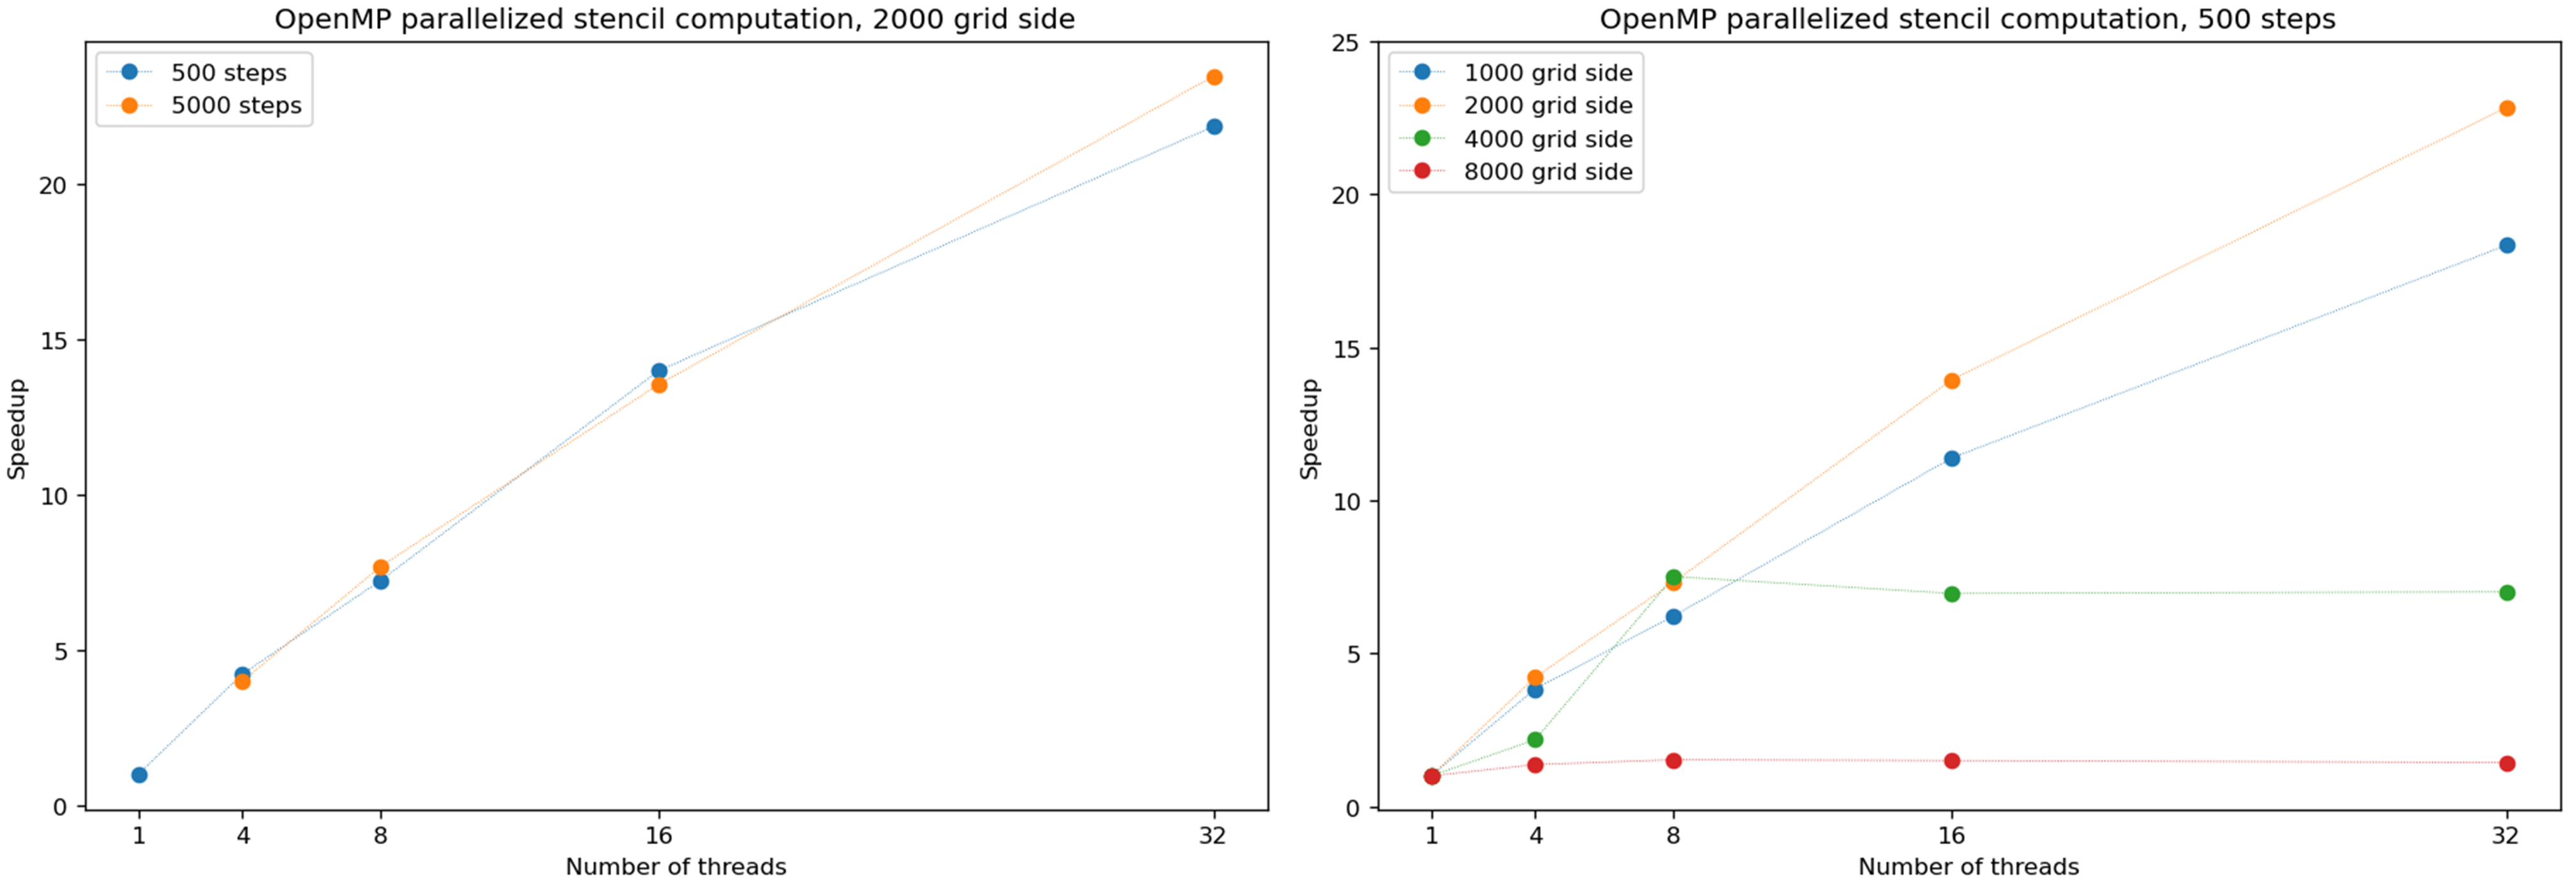
\includegraphics[width=0.9\textwidth]{fig_problem/heat_omp_step_gridside.png}
\caption{OpenMP parallelized stencil computations. Left for the computations with 2000 grid size at varied steps, and right for computations at 500 steps with varied number of grid side.}\label{fig:heat_omp_step_gridside}
\end{figure}


\par
A short summary of the heat flow computation scaling program.
\begin{itemize}
    \item The heat flow computation exhibits linear scaling behavior with respect to the number of time steps. Since each time-step update is sequential and involves a similar number of operations, the update time will be more or less constant.
    \item The stencil application (grid update) is expected to exhibit quadratic scaling character respect to the size of grid side. Since stencil application is independent for every grid point, the update time will be proportional to the number of points ($i.e.$, side * side).
    \item The GPU-accelerated computations are expected to suffer from the memory effect. GPU computations are indeed sensitive to memory access patterns and tend to resort to (GPU) memory quickly. However, the effect above arises because multiple active CPU threads start competing for access to RAM. In contrast,|\lq\lq over-subscribing\rq\rq~the GPU with large amount of threads executing the same kernel (stencil update on a grid point) tends to hide memory access latencies; increasing grid size might actually help to achieve this.
\end{itemize}


% ---------------------------------------------------------------------- %


\subsection{GPU parallelization}


\subsubsection{Porting sequential C++ code to naive GPU parallelization}


\par
Let’s apply several techniques presented in previous sections to make stencil update (List~\ref{lst:13_heat_diffusion_stencil_cpu_update}) GPU-parallel.
The OpenMP (or OpenACC) offloading requires to define a region to be executed in parallel as well as data that shall be copied over/used in GPU memory.
Similarly, the SYCL programming model offers convenient ways to define execution kernels, context to run them in (called queue) and simplified CPU-GPU transfer of needed data.
Changes of stencil update code shown in List~\ref{lst:13_heat_diffusion_stencil_cpu_update} for OpenMP and SYCL are shown in List~\ref{lst:13_heat_diffusion_stencil_gpu_openmp_naive} and List~\ref{lst:13_heat_diffusion_stencil_gpu_sycl_naive}, respectively.


\lstinputlisting[language=c++, caption={Changes of stencil update scheme shown in List~\ref{lst:13_heat_diffusion_stencil_cpu_update} in C++ for GPU programming using OpenMP.}, label={lst:13_heat_diffusion_stencil_gpu_openmp_naive}, xleftmargin=0.05\textwidth, xrightmargin=0.05\textwidth]{code_examples/13_heat_diffusion_stencil_gpu_openmp_naive.cpp}


\lstinputlisting[language=c++, caption={Changes of stencil update scheme shown in List~\ref{lst:13_heat_diffusion_stencil_cpu_update} in C++ for GPU programming using SYCL.}, label={lst:13_heat_diffusion_stencil_gpu_sycl_naive}, xleftmargin=0.05\textwidth, xrightmargin=0.05\textwidth]{code_examples/13_heat_diffusion_stencil_gpu_sycl_naive.cpp}


\subsubsection{Compiling SYCL executables}


\par
As SYCL is placed on top of ROCm/HIP (or CUDA) software stack, even running SYCL executables may require respective modules to be loaded.
On the LUMI-G nodes, it can be done as follows.
\lstinputlisting[language=bash, firstline=10, lastline=16, label={lst:13_heat_diffusion_stencil_path}, xleftmargin=0.05\textwidth, xrightmargin=0.05\textwidth]{code_examples/13_heat_diffusion_stencil_path.pbs}


\par
As described in previous sections, you can generate your own executables.
This time we will use the interactive allocation for GPU computing.
\lstinputlisting[language=bash, firstline=24, lastline=31, label={lst:13_heat_diffusion_stencil_path}, xleftmargin=0.05\textwidth, xrightmargin=0.05\textwidth]{code_examples/13_heat_diffusion_stencil_path.pbs}


\par
In the interactive allocation, run (using~\textbf{\textcolor{brown}{srun}}) provided or compiled executables~\textbf{\textcolor{brown}{base/stencil}},~\textbf{\textcolor{brown}{base/stencil\_off}} and~\textbf{\textcolor{brown}{sycl/stencil\_naive}}.
Try changing problem size parameters~\textbf{\textcolor{brown}{srun stencil\_naive 2000 2000 5000}} to see how computation time changes.


\subsubsection{Timing naive GPU parallelization}


\par
If you ran the code examples mentioned above for the heat diffusion program, you might already know that the GPU-\lq\lq ported\rq\rq~versions actually run slower than the single-CPU-core version.
In fact, the scaling behavior of all three variants is similar and expected, which is a good sign; only the~\lq\lq computation unit cost\rq\rq~is different.
You can compare benchmark summaries shown in Fig.~\ref{fig:heat_seq_openmp_sycl_naive}.


\begin{figure}[!htbp]
\centering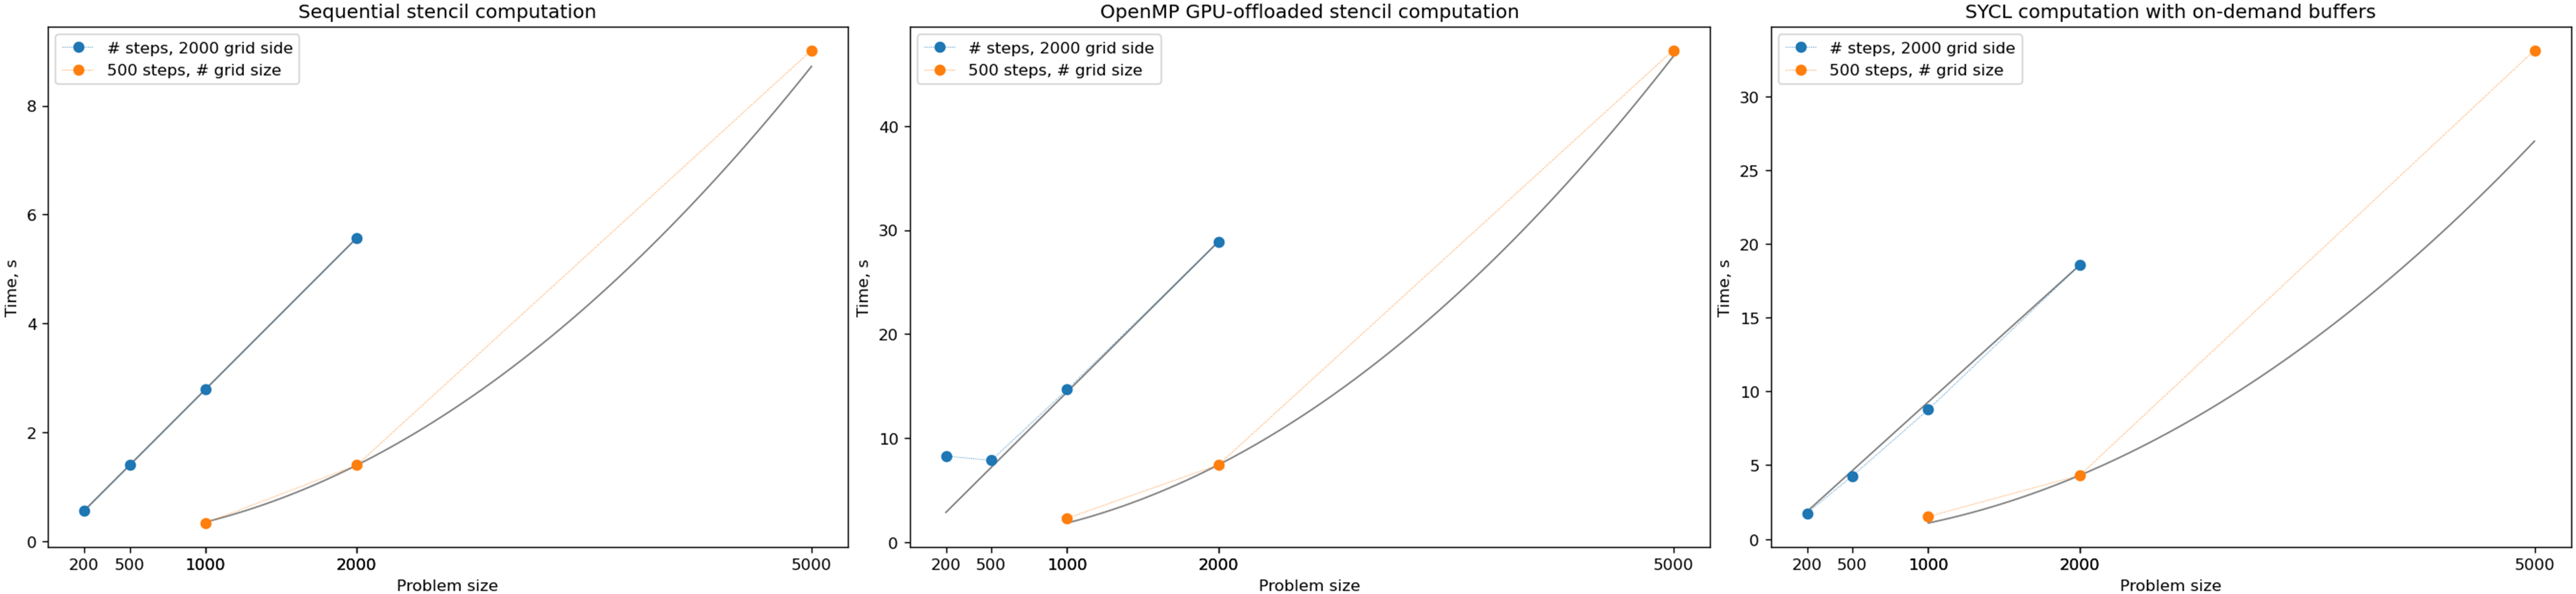
\includegraphics[width=0.9\textwidth]{fig_problem/heat_seq_openmp_sycl_naive.png}
\caption{Sequential and parallelized stencil computations. Left for the sequential stencil computations, middle for OpenMP GPU-offloaded stencil computations, and right for SYCL computations with on-demand buffers.}\label{fig:heat_seq_openmp_sycl_naive}
\end{figure}


\subsubsection{Data movement in GPU parallelization}


\par
Why the GPU-ported versions above seem to be grossly inefficient? At each step, we follow the right procedures for GPU progrmming: 1) re-allocate GPU memory; 2) copy data from CPU to GPU; 3) perform GPU computations; and 4) copy data back from GPU to CPU.
It was revealed that the steps for copying data from CPU to GPU and back are the most time consuming part during the code execution.
In fact the overhead can be reduced by taking following steps to minimize data transfers between host (CPU) and device (GPU) memory: 1) allocate GPU memory once at the start of the program; 2) only copy data from GPU to CPU when we need it; and 3) swap GPU buffers between timesteps, like we do with CPU buffers (OpenMP does this automatically).
As such, we can upgrade the stencil update code for OpenMP (List~\ref{lst:13_heat_diffusion_stencil_gpu_openmp_naive}) and SYCL (List~\ref{lst:13_heat_diffusion_stencil_gpu_sycl_naive}), and the obtained stencil update code are available at List~\ref{lst:13_heat_diffusion_stencil_gpu_openmp_naive_update} and List~\ref{lst:13_heat_diffusion_stencil_gpu_sycl_naive_update} for OpenMP and SYCL, respectively.
In addition, the main function for SYCL is provided in List~\ref{lst:13_heat_diffusion_stencil_gpu_sycl_naive_update_main}, and a naive version for Python is also provided in List~\ref{lst:13_heat_diffusion_stencil_gpu_python_naive} for a comparative purpose.


\lstinputlisting[language=c++, caption={Changes of stencil update scheme shown in List~\ref{lst:13_heat_diffusion_stencil_gpu_openmp_naive} for naive GPU parallelization using OpenMP.}, label={lst:13_heat_diffusion_stencil_gpu_openmp_naive_update}, xleftmargin=0.05\textwidth, xrightmargin=0.05\textwidth]{code_examples/13_heat_diffusion_stencil_gpu_openmp_naive_update.cpp}


\lstinputlisting[language=c++, caption={Changes of stencil update scheme shown in List~\ref{lst:13_heat_diffusion_stencil_gpu_sycl_naive} for naive GPU parallelization using SYCL.}, label={lst:13_heat_diffusion_stencil_gpu_sycl_naive_update}, xleftmargin=0.05\textwidth, xrightmargin=0.05\textwidth]{code_examples/13_heat_diffusion_stencil_gpu_sycl_naive_update.cpp}


\lstinputlisting[language=c++, caption={The main function for naive GPU parallelization using SYCL.}, label={lst:13_heat_diffusion_stencil_gpu_sycl_naive_update_main}, xleftmargin=0.05\textwidth, xrightmargin=0.05\textwidth]{code_examples/13_heat_diffusion_stencil_gpu_sycl_naive_update_main.cpp}


\lstinputlisting[language=python, caption={The main function for naive GPU parallelization using Python.}, label={lst:13_heat_diffusion_stencil_gpu_python_naive}, xleftmargin=0.05\textwidth, xrightmargin=0.05\textwidth]{code_examples/13_heat_diffusion_stencil_gpu_python_naive.py}


\subsubsection{Timing updated GPU parallelization}


\par
Again, we can run (using~\textbf{\textcolor{brown}{srun}}) the provided or compiled executables~\textbf{\textcolor{brown}{base/stencil\_data}} and~\textbf{\textcolor{brown}{sycl/stencil}} in the interactive allocation.
Try changing problem size parameters~\textbf{\textcolor{brown}{srun stencil 2000 2000 5000}} to see how computation time changes.


\par
Fig.~\ref{fig:heat_openmp_sycl_update} provides the output for these updated GPU computations.
Using GPU offloading with mapped GPU data, it is possible to achieve performance gains compared to the thread-parallel CPU version for larger grid sizes, due to the fact that the latter version becomes essentially RAM-bound, but the former does not.
In addition, because of the more explicit programming approach, SYCL GPU port is still 10 times faster than OpenMP offloaded version, comparable with thread-parallel CPU version running on all cores of a single node. Moreover, the performance scales perfectly with respect to both the grid size and the number of time steps (grid updates) computed.


\begin{figure}[htbp]
\centering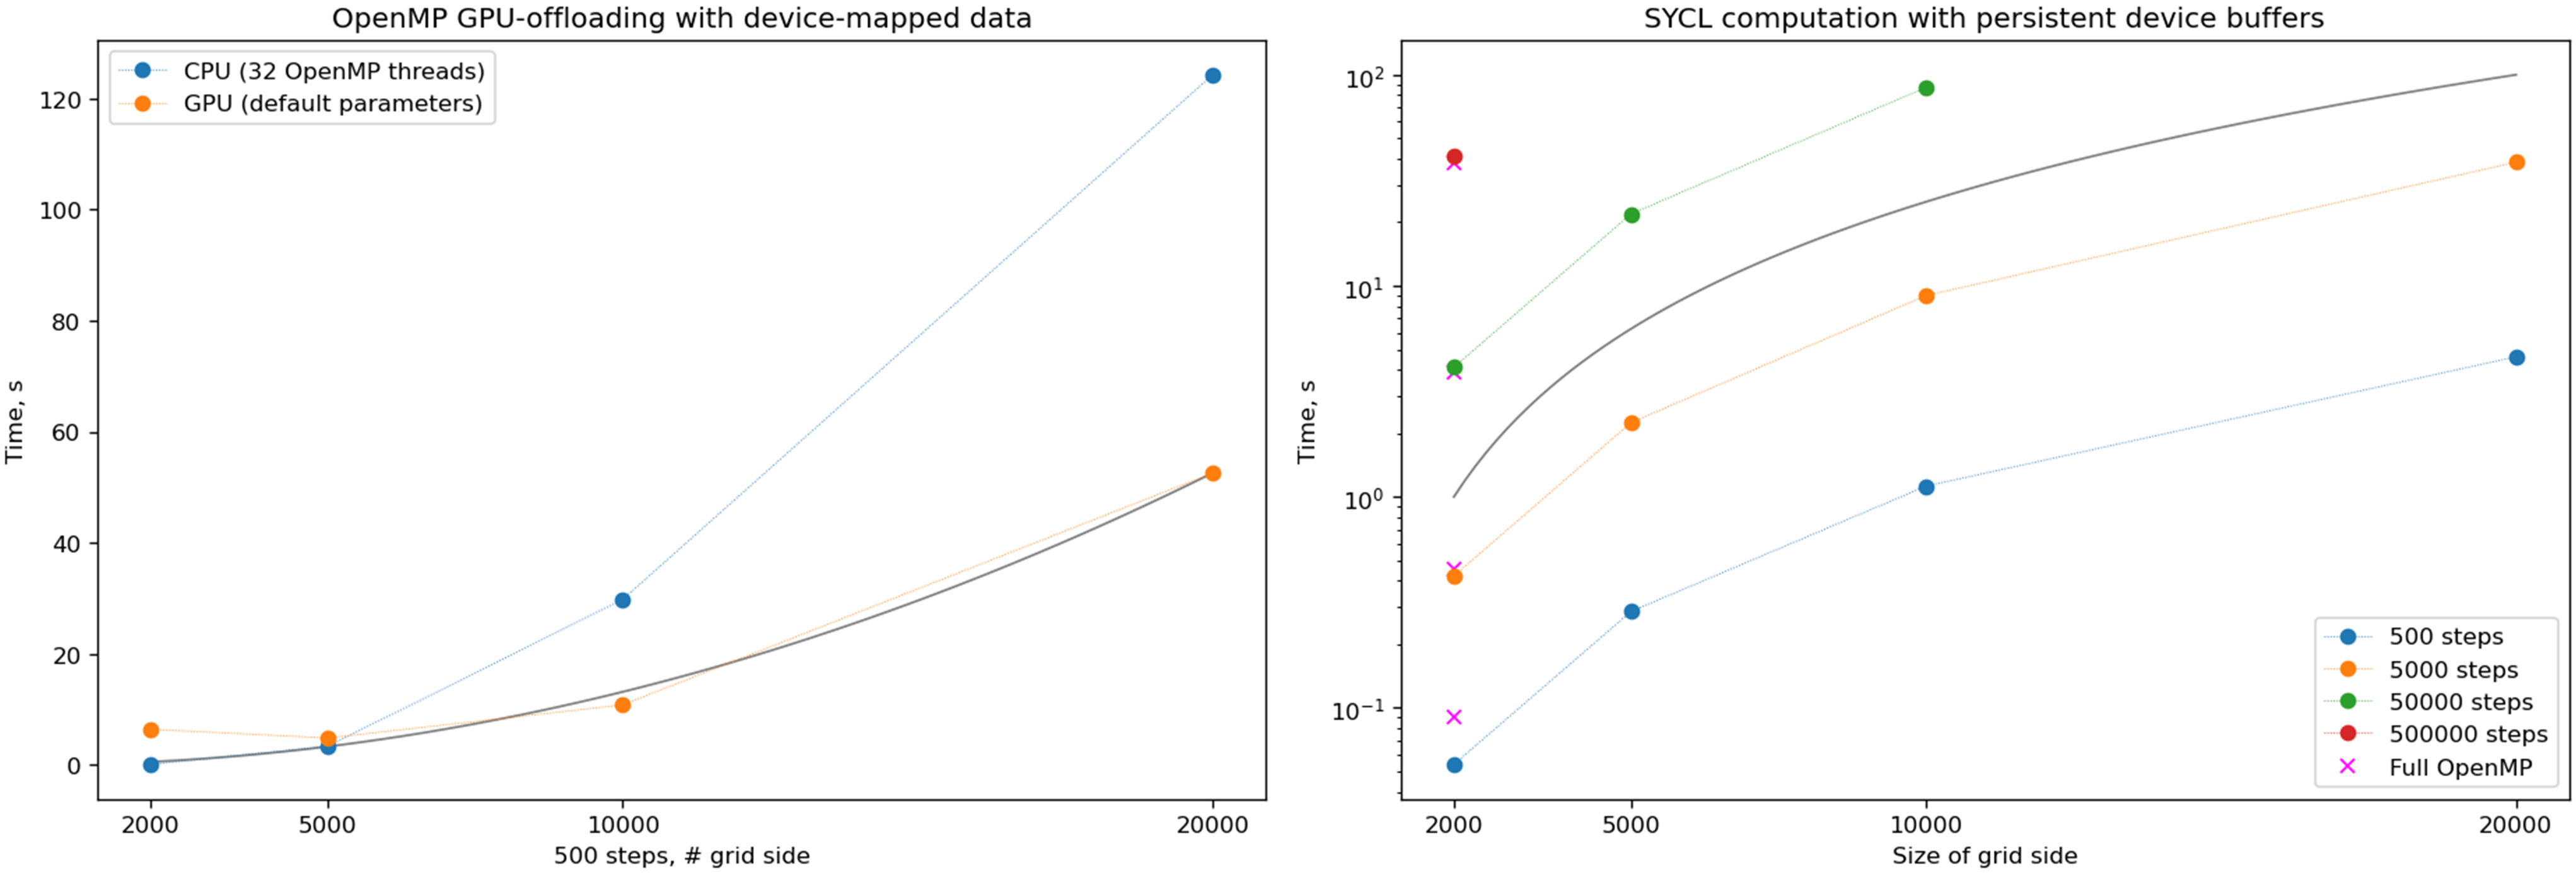
\includegraphics[width=0.9\textwidth]{fig_problem/heat_openmp_sycl_update.png}
\caption{Updated GPU parallelized stencil computations. Left for OpenMP GPU-offfloading with device-mapped data, and right fore SYCL GPU computation with persistent device buffers.}\label{fig:heat_openmp_sycl_update}
\end{figure}


% ---------------------------------------------------------------------- %


\subsection{Python: JIT and GPU acceleration}


\subsubsection{JIT acceleration in Python}


\par
As mentioned in previous subsections, the~\textbf{Numba} package allows developers to \textbf{JIT} compile Python code to run fast on CPUs, but can also be used for JIT compiling for GPUs (although AMD GPU support is at the moment deprecated for Numba versions $>$ 0.53).
JIT seems to work well on loop-based, computationally heavy functions, so trying it out is a nice choice for initial source version.
The code examples for the stencil update scheme and the data generation function are provided in List~\ref{lst:13_heat_diffusion_stencil_gpu_python_jit_stencil_update} and List~\ref{lst:13_heat_diffusion_stencil_gpu_python_jit_data_generation}, respectively.


\lstinputlisting[language=python, caption={The stencil update scheme for Python GPU parallelization using JIT in Numba.}, label={lst:13_heat_diffusion_stencil_gpu_python_jit_stencil_update}, xleftmargin=0.05\textwidth, xrightmargin=0.05\textwidth]{code_examples/13_heat_diffusion_stencil_gpu_python_jit_stencil_update.py}


\lstinputlisting[language=python, caption={The data generation function for Python GPU parallelization using JIT in Numba.}, label={lst:13_heat_diffusion_stencil_gpu_python_jit_data_generation}, xleftmargin=0.05\textwidth, xrightmargin=0.05\textwidth]{code_examples/13_heat_diffusion_stencil_gpu_python_jit_data_generation.py}


\par
The alternative approach would be to rewrite stencil update code in NumPy style, exploiting loop vectorization.
You can try to run the provided Python examples using the Google Colab with instructions provided in the~\href{https://enccs.github.io/gpu-programming/0-setup/#running-on-google-colab}{Setup} on your local machine or LUMI node (non-GPU variants).
On LUMI, you can set up Python distribution as following:
\lstinputlisting[language=bash, firstline=40, lastline=47, label={lst:13_heat_diffusion_stencil_path}, xleftmargin=0.05\textwidth, xrightmargin=0.05\textwidth]{code_examples/13_heat_diffusion_stencil_path.pbs}


\par
A short summary of a typical Colab run is provided in Table~\ref{tbl:gpu_python_google_colab}. 
For later comparison, some benchmarks of the thread-parallel executable are provided in Table~\ref{tbl:gpu_python_google_colab}.


\begin{table}[!h]
\centering\caption{Run times of Numba JIT-enabled Python program in second.}\label{tbl:gpu_python_google_colab}
\begin{tabular}{ |c|c|c|c|c| } 
\hline
\textbf{Job size} & \textbf{JIT (LUMI)} & \textbf{JIT (Colab)} & \textbf{Job size} & \textbf{no JIT (Colab)} \\
\hline
S:2000 T:500 & 1.648 & 8.495 & S:200 T:50 & 5.318 \\
S:2000 T:200 & 0.787 & 3.524 & S:200 T:20 & 1.859 \\
S:1000 T:500 & 0.547 & 2.230 & S:100 T:50 & 1.156 \\
\hline
\end{tabular}
\end{table}


\par
Numba’s~\textbf{\textcolor{red}{@vectorize}} and~\textbf{\textcolor{red}{@guvectorize}} decorators offer an interface to create CPU- (or GPU-) accelerated Python functions without explicit implementation details.
However, such functions become increasingly complicated to write (and optimize by the compiler) with increasing complexity of the computations within.


\par
For NVIDIA GPUs, Numba also offers direct CUDA-based kernel programming, which can be the best choice for those already familiar with CUDA.
An example for stencil update written in Numba CUDA is shown in List~\ref{lst:13_heat_diffusion_stencil_gpu_python_naive}.
In this case, the data transfer functions~\textbf{\textcolor{red}{devdata = cuda.to\_device(data)}} and~\textbf{\textcolor{red}{devdata.copy\_to\_host(data)}} shown in the~\textbf{\textcolor{brown}{main\_cuda.py}} are already provided by the Numba package.


\subsubsection{CUDA acceleration in Python}


\par
Using the Google Colab (or your own machine), run provided Numba-CUDA Python program.
Try to change problem size parameters and rerun the computations:
\begin{itemize}
    \item \textbf{\textcolor{brown}{args.rows, args.cols, args.nsteps = 2000, 2000, 5000}} for notebooks.
    \item \textbf{\textcolor{brown}{srun python3 main.py 2000 2000 5000}} for command line.
\end{itemize}


\par
The obtained numbers from Google Colab are listed in Table~\ref{tbl:gpu_python_google_colab_numba}.


\begin{table}[!h]
\centering\caption{Run times of Numba CUDA Python program in second.}\label{tbl:gpu_python_google_colab_numba}
\begin{tabular}{ |c|c|c|c| } 
\hline
\textbf{Job size} & \textbf{JIT (LUMI)} & \textbf{JIT (Colab)} & \textbf{CUDA (Colab)} \\
\hline
S:2000 T:500 & 1.648 & 8.495 & 1.079 \\
S:2000 T:2000 & 6.133 & 36.61 & 3.931 \\
S:5000 T:500 & 9.478 & 57.19 & 6.448 \\
\hline
\end{tabular}
\end{table}


% ---------------------------------------------------------------------- %


\subsection{Julia acceleration}


\subsubsection{Julia code for CPU}


\par
A Julia version of the stencil example discussed above can be found below.
A simplified version of the HeatEquation module is provided at the~\href{https://github.com/ENCCS/HeatEquation.jl}{ENCCS repository}.
The source files are also available in the~\textbf{\textcolor{brown}{content/examples/stencil/julia}} subdirectory of this repository~\cite{gpu-programming-examples}.


\par
To run the example on the LUMI CPU partition, you should the following commands:
\lstinputlisting[language=bash, firstline=57, lastline=69, label={lst:13_heat_diffusion_stencil_path}, xleftmargin=0.05\textwidth, xrightmargin=0.05\textwidth]{code_examples/13_heat_diffusion_stencil_path.pbs}


\par
To run the example on the LUMI GPU partition, use instead the command below:
\lstinputlisting[language=bash, firstline=78, lastline=78, label={lst:13_heat_diffusion_stencil_path}, xleftmargin=0.05\textwidth, xrightmargin=0.05\textwidth]{code_examples/13_heat_diffusion_stencil_path.pbs}


\par
The code examples consisting of~\textbf{\textcolor{brown}{main.jl}},~\textbf{\textcolor{brown}{core.jl}},~\textbf{\textcolor{brown}{heat.jl}}, and~\textbf{\textcolor{brown}{project.toml}} are provided in List~\ref{lst:13_heat_diffusion_julia_main}, List~\ref{lst:13_heat_diffusion_julia_core}, List~\ref{lst:13_heat_diffusion_julia_heat}, and List~\ref{lst:13_heat_diffusion_julia_proj}, respectively.


\lstinputlisting[language=c++, caption={The~\textbf{\textcolor{brown}{main.jl}} file for the heat diffusion program in Julia.}, label={lst:13_heat_diffusion_julia_main}, xleftmargin=0.05\textwidth, xrightmargin=0.05\textwidth]{code_examples/13_heat_diffusion_julia_main.jl}


\lstinputlisting[language=c++, caption={The~\textbf{\textcolor{brown}{core.jl}} file for the heat diffusion program in Julia.}, label={lst:13_heat_diffusion_julia_core}, xleftmargin=0.05\textwidth, xrightmargin=0.05\textwidth]{code_examples/13_heat_diffusion_julia_core.jl}


\lstinputlisting[language=c++, caption={The~\textbf{\textcolor{brown}{heat.jl}} file for the heat diffusion program in Julia.}, label={lst:13_heat_diffusion_julia_heat}, xleftmargin=0.05\textwidth, xrightmargin=0.05\textwidth]{code_examples/13_heat_diffusion_julia_heat.jl}


\lstinputlisting[language=c++, caption={The~\textbf{\textcolor{brown}{project.toml}} file for the heat diffusion program in Julia.}, label={lst:13_heat_diffusion_julia_proj}, xleftmargin=0.05\textwidth, xrightmargin=0.05\textwidth]{code_examples/13_heat_diffusion_julia_project.toml}


\par
Note that the~\textbf{\textcolor{brown}{plots.jl}} dependency is commented out in~\textbf{\textcolor{brown}{main.jl}} (the 1$^{st}$, 35-36, and 41-42 lines in List~\ref{lst:13_heat_diffusion_julia_main}) and~\textbf{\textcolor{brown}{project.toml}} (the 3$^{rd}$ line in List~\ref{lst:13_heat_diffusion_julia_proj}) files.
This saves ~2 minute precompilation time when you first instantiate the Julia environment.
To generate plots, just uncomment the commented~\textbf{\textcolor{brown}{plots.jl}} dependency in the~\textbf{\textcolor{brown}{project.toml}} file (List~\ref{lst:13_heat_diffusion_julia_proj}), instantiate again, and import and use~\textbf{\textcolor{brown}{Plots}} in the~\textbf{\textcolor{brown}{main.jl}} file (List~\ref{lst:13_heat_diffusion_julia_main}).


\subsubsection{Julia port to GPU}


\par
Carefully inspect all Julia source files and consider the following questions:
\begin{itemize}
    \item Which functions should be ported to run on GPU?
    \item Look at the $initialize!()$ function and how it uses the $arraytype$ argument. This could be done more compactly and elegantly, but this solution solves scalar indexing errors. What are scalar indexing errors?
    \item Try to start sketching GPU-ported versions of the key functions.
    \item When you have a version running on a GPU (your own or the solution provided below), try benchmarking it by adding~\textbf{\textcolor{red}{@btime}} in front of $simulate!()$ in the~\textbf{\textcolor{brown}{main.jl}} file. Benchmark also the CPU version, and compare the obtained computational results.
\end{itemize}


\par
Some simple hints are provided below:
\begin{itemize}
    \item create a new function $evolve\_gpu!()$ which contains the GPU kernelized version of $evolve!()$;
    \item in the loop over timesteps in $simulate!()$, you will need a conditional like $if typeof(curr.data) <: ROCArray$ to call your GPU-ported functional;
    \item you cannot pass the struct $Field$ to the kernel. You will instead need to directly pass the array $Field.data$. This also necessitates passing in other variables like $curr.dx^2$, $etc$.
\end{itemize}


\par
More hints to upgrade the code for GPU acceleration using Julia are listed here.
\begin{itemize}
    \item since the data is two-dimensional, you’ll need $i = (blockIdx().x - 1) * blockDim().x + threadIdx().x$ and $j = (blockIdx().y - 1) * blockDim().y + threadIdx().y$;
    \item not to overindex the 2D array, you can use a conditional like $if~i>1~\&\&~j > 1~\&\&~i < nx+2~\&\&~j < ny+2$;
    \item when calling the kernel, you can set the number of threads and blocks like $xthreads = ythreads = 16$ and $xblocks, yblocks = cld(curr.nx, xthreads), cld(curr.ny, ythreads)$.
    \item call it with the command, $e.g.$, $@roc~threads=$ $(xthreads, ythreads) blocks=$ $(xblocks, yblocks)$ $evolve\_rocm!(curr.data,prev.data,curr.dx^2,curr.dy^2,nx,ny,a,dt)$.
\end{itemize}


\par
The solution for GPU acceleration using Julia are described below, and the code examples of~\textbf{\textcolor{brown}{main\_gpu.jl}} and~\textbf{\textcolor{brown}{core\_gpu.jl}} are provided in List~\ref{lst:13_heat_diffusion_julia_main_gpu} and List~\ref{lst:13_heat_diffusion_julia_core_gpu}, respectively.
\begin{itemize}
    \item The $evolve!()$ and $simulate!()$ functions need to be ported. The~\textbf{\textcolor{brown}{main.jl}} (List~\ref{lst:13_heat_diffusion_julia_main}) file also needs to be updated to work with GPU arrays.
    \item \lq\lq Scalar indexing\rq\rq~is the place where you iterate over a GPU array, which would be excruciatingly slow and is indeed only allowed in interactive REPL sessions. Without the if-statements in the $initialize!()$ function, the $generate\_field!()$ method would be doing disallowed scalar indexing if you were running on a GPU.
    \item The GPU-ported version is found below. Try it out on both CPU and GPU and observe the speedup. Play around with array size to see if the speedup is affected. You can also play around with the $xthreads$ and $ythreads$ variables to see if it changes anything.
\end{itemize}


\lstinputlisting[language=c++, caption={The~\textbf{\textcolor{brown}{main\_gpu.jl}} file for GPU acceleration of the heat diffusion program in Julia.}, label={lst:13_heat_diffusion_julia_main_gpu}, xleftmargin=0.05\textwidth, xrightmargin=0.05\textwidth]{code_examples/13_heat_diffusion_julia_main_gpu.jl}


\lstinputlisting[language=c++, caption={The~\textbf{\textcolor{brown}{core\_gpu.jl}} file for GPU acceleration of the heat diffusion program in Julia.}, label={lst:13_heat_diffusion_julia_core_gpu}, xleftmargin=0.05\textwidth, xrightmargin=0.05\textwidth]{code_examples/13_heat_diffusion_julia_core_gpu.jl}


\par
In summary, this section leans heavily on source code and material created for several other computing workshops by~\href{https://enccs.se/}{ENCCS} and~\href{https://www.csc.fi/en/home}{CSC} and adapted for the purposes of this lesson.
If you want to know more about specific programming models/framework, definitely check the reading materials below.
\begin{itemize}
    \item~\href{https://enccs.github.io/openmp-gpu/}{OpenMP for GPU offloading}
    \item~\href{https://enccs.github.io/sycl-workshop/}{Heterogeneous programming with SYCL}
    \item~\href{https://github.com/cschpc/heat-equation/}{Educational implementation of heat flow example} (incl. MPI-aware CUDA)
\end{itemize}
